\subsection{The decision of parameter $\tau$}
\label{sec:decision_tau}
One parameter of AC is the overlap constraint $\tau$.
%we should decide it in order to carry on the next potential applications.
To decide the value of $\tau$, we compute
$F_1$ score for the different settings of $\tau$ (from $0.05$ to $0.5$)
by setting $k=10$ for Verb-20.
\figref{fig:f1_vs_tau} shows the distribution of the maximum $F_1$ score against $\tau$.
Each point stands for a verb in Verb-20.
In the figure, we observe that by setting $\tau$ from $0.1$ to $0.25$, we can obtain an optimal
result for most verbs.
We further calculate the deviation of the $F_1$ score at $\tau=0.2$
from the maximum $F_1$ score for each verb, i.e.,
\[dev(v) = F_1(v)_{max} - F_1(v)_{\tau=0.2},\] 
and plot the distribution of these deviations on all 20 verbs 
in \figref{fig:variance}.
The figure shows that most of verbs achieve maximum $F_1$ score
or are very close to the maximum $F_1$ when setting $\tau=0.2$.
Therefore, for simplicity, we set $\tau=0.2$ for all subsequent experiments.

%\begin{figure}[th]
%\centering
%\epsfig{file=figure/f1_vs_tau.eps,width=.65\columnwidth}
%\vspace*{-2ex}
%\caption{$F1_{max}$ against $\tau$}
%\label{fig:f1_vs_tau}
%\end{figure}
\begin{figure}[th]
\begin{minipage}[t]{0.49\columnwidth}
\centering
\epsfig{file=figure/f1_vs_tau.eps,width=\columnwidth}
\caption{Maximum $F_1$ against $\tau$}
\label{fig:f1_vs_tau}
\end{minipage}
\hfill
\begin{minipage}[t]{0.49\columnwidth}
\centering
\epsfig{file=figure/variance.eps,width=\columnwidth}
\caption{Distribution of deviation from $F_1(v)_{max}$}
\label{fig:variance}
\end{minipage}
\end{figure}

%\begin{table}[th]
%\caption{The deviation between $F_1(\tau=0.2)$ to the maximum $F_1$}
%\center
%\small
%\begin{tabular}{|l|l|l|l|l|}
%\hline
%bring&carry&connect&cut&define\\
%\hline
%0.01 & 0.02 & 0.02 & 0.04 & 0.04\\
%\hline
%eat&help&hit&keep&operate\\
%\hline
%0.05 & 0.00 & 0.03 & 0.00 & 0.00\\
%\hline
%perform&play&read&release&report\\
%\hline
%0.02 & 0.00 & 0.04 & 0.03 & 0.02\\
%\hline
%select&spend&submit&visit&wear\\
%\hline
%0.00 & 0.05 & 0.00 & 0.00 & 0.01\\
%\hline
%\end{tabular}
%\label{tab:f1_deviation}
%\end{table}
